% Provenance (never printed): see sources/outline_sources.md (Year 3:
% speciation and saturation indices; carbonate equilibria applied to rocks;
% weathering kinetics; hydrothermal fluids). Brief: sources/book5/BRIEFS.md,
% ch. 15. Curves from figdata/bachelor-3/carbonate_system.py,
% activity_diagram.py, weathering_rates.py. Exercise and problem values in the
% Book 5 scratch calculator calc/ch15.py. The spring below the Varden
% limestone, its analysis and the granite stream are invented.
\chapter{水–岩相互作用}\label{ch:b3:water-rock-interaction}

位于石灰岩陡崖脚下的一处泉水，在它接触的每一根
枝条和每一块石头上都留下一层白色结壳；流经花岗岩的
一条溪流携带二氧化硅、钠和少量钾，却完全不留下结壳。
两者的差别在于水的化学成分，而化学成分记录了水
所流经岩石的历史：它携带了多少二氧化碳，停留了多久，
溶解了哪些矿物，又形成了哪些矿物。本章借助溶液化学的工具
读取这一记录，内容从水的分析，到矿物溶解速率，
再到地壳中热流体的同位素示踪。

\begin{recall}
活度、活度系数、离子强度、化学形态、溶度积、
碱度、饱和度 $\Omega$、亨利定律、速率方程、
阿伦尼乌斯定律、过渡态和 $\delta$ 值，
都在化学学科的大学分册中。化学风化、硅酸盐的水解、黏土矿物和高岭石，
见本科一年级分册中关于风化与黏土的一章；
溶跃面和碳酸盐补偿深度，见其中关于碳酸盐、硅质
和蒸发岩沉积的一章。热液流体见本科二年级分册
中关于矿床的一章，硅酸盐风化恒温器见其中关于
地质时间气候的一章；
热液循环则见于中学教材。
\end{recall}

\section{天然水的分析}\label{sec:b3:water-rock-interaction:analysis}

一份水分析以毫克每升为单位列出主要离子：钙、
镁、钠和钾；碳酸氢根、氯离子、硫酸根和硝酸根；
以 \ce{SiO2} 计的溶解硅；以及在水源处测定的 pH 值和温度，
因为样品离开水源后两者都会改变。以摩尔质量除浓度，
得到以毫摩尔每升计的浓度，再乘以电荷数，
得到毫当量每升。低矿化度水呈电中性，因此
阳离子之和必等于阴离子之和。

\begin{method}[水分析的检验]\label{met:b3:water-rock-interaction:analysis}
\begin{enumerate}
\item 将各浓度换算为 \unit{mmol/L} 与 \unit{meq/L}；
\item 以 \unit{meq/L} 计，分别求阳离子与阴离子之和；
\item 计算电荷平衡误差 $100\,(\sum\text{阳离子} -
  \sum\text{阴离子})/(\sum\text{阳离子} + \sum\text{阴离子})$，以百分数表示；
\item 对于 250 至 \qty{1000}{mg/L} 的水，若误差在 1 或 \qty{2}{\percent} 以内，则接受该分析；
  对于更稀的水，误差允许略大；
  否则应查找遗漏的离子或分析误差。
\end{enumerate}
\end{method}
% ledger: hem85:charge-balance

离子的活度等于其质量摩尔浓度乘以活度系数
$\gamma$。天然水中的 $\gamma$ 由离子强度 $I =
\tfrac12\sum m_i z_i^2$，按扩展的德拜–休克尔方程计算
\[
-\log\gamma_i = \frac{A z_i^2\sqrt I}{1 + B a_i\sqrt I},
\]
对于 \qty{25}{\celsius} 的水，$A = 0.5085$，$B = 0.3281$，离子尺寸
$a_i$ 以埃为单位，\ce{H+} 为 9，\ce{Mg^2+} 为 8，\ce{Ca^2+} 为 6，
\ce{CO3^2-} 为 5，\ce{Na+}、\ce{HCO3-} 和 \ce{SO4^2-} 为 4，
\ce{K+}、\ce{Cl-}、\ce{OH-} 和 \ce{NO3-} 为 3。该方程适用于
一价盐浓度约为 \qty{0.1}{mol/L} 以内的情形，可用于河流和大多数
地下水，但不适用于海水或卤水。温度仅使 $A$ 在
\qty{0}{\celsius} 时的 0.4883 与 \qty{60}{\celsius} 时的 0.5425 之间变化，
因此 \qty{25}{\celsius} 下的数值对低温水同样适用。
% ledger: hem85:debye-huckel

水中的无机碳分配于溶解的二氧化碳
（\ce{CO2} 表示 \ce{CO2} 与 \ce{H2CO3} 之和）、碳酸氢根与碳酸根之间，
三者由下列关系式联系：
\[
K_1 = \frac{a_{\ce{HCO3-}}\,a_{\ce{H+}}}{a_{\ce{CO2}}}, \qquad
K_2 = \frac{a_{\ce{CO3^2-}}\,a_{\ce{H+}}}{a_{\ce{HCO3-}}}, \qquad
K_H = \frac{a_{\ce{CO2}}}{P_{\ce{CO2}}},
\]
在 \qty{25}{\celsius} 下，$\log K_1 = -6.35$，$\log K_2 = -10.33$，
$\log K_H = -1.47$；在 \qty{10}{\celsius} 下，三者分别为 $-6.46$、$-10.49$ 和 $-1.27$
（$P$ 以大气压计）。在 pH 6.4 至 10.3 之间碳酸氢根占主导，多数天然水的碱度几乎全部来自碳酸氢根。
由实测的 pH 值和碳酸氢根浓度，
可求出另外两种物种的浓度，以及
水与之达到平衡的二氧化碳分压。
% ledger: phreeqc:carbonate

\section{饱和}\label{sec:b3:water-rock-interaction:saturation}

\begin{definition}[饱和指数]\label{def:b3:water-rock-interaction:si}
称水中某矿物的\emph{饱和指数}\index{饱和指数}为
$\mathrm{SI} = \log(\mathrm{IAP}/K)$，其中 IAP 为水的离子活度积，
其写法与该矿物的溶度积 $K$ 相同，
即 $\mathrm{SI} = \log\Omega$。
\end{definition}

若 $\mathrm{SI} < 0$，水可溶解该矿物；若 $\mathrm{SI} > 0$，水可使其沉淀，
而 $\mathrm{SI} = 0$ 表示平衡。
由于溶解反应的自由能为 $\Delta_r G = RT\ln\Omega
= 2.303\,RT\,\mathrm{SI}$，\omterm{def:b3:water-rock-interaction:si}{饱和指数}也是驱动力的度量，
其单位为 $2.303\,RT$，在 \qty{25}{\celsius} 时约为 \qty{5.7}{kJ/mol}。
对于方解石，$\mathrm{IAP} = a_{\ce{Ca^2+}}
a_{\ce{CO3^2-}}$，且在 \qty{25}{\celsius} 时 $\log K = -8.45$，在 \qty{10}{\celsius} 时为 $-8.35$，
说明方解石在冷水中溶解度更大。对于石膏，$\mathrm{SI} = \log(a_{\ce{Ca^2+}}a_{\ce{SO4^2-}}) + 4.55$；
对于石英，其溶解生成中性的 \ce{H4SiO4}，$\mathrm{SI} = \log
a_{\ce{H4SiO4}} + 3.98$，而对于无定形二氧化硅，常数为 2.71
而非 3.98。实测指数的不确定度至少为 $\pm0.1$，
指数在 $\pm0.3$ 以内的水被视为接近平衡。
% ledger: phreeqc:carbonate, phreeqc:silicates, hem85:si

\section{岩石中的碳酸盐平衡}\label{sec:b3:water-rock-interaction:carbonate}

方解石在溶有二氧化碳的水中按下式溶解
\[
\ce{CaCO3 + CO2 + H2O <=> Ca^2+ + 2 HCO3-},
\qquad K = \frac{a_{\ce{Ca^2+}}\,a_{\ce{HCO3-}}^2}{P_{\ce{CO2}}}
= \frac{K_{\mathrm{cal}}K_1K_H}{K_2},
\]
在 \qty{25}{\celsius} 时 $\log K = -5.94$，在 \qty{10}{\celsius} 时为 $-5.59$。
溶解量取决于二氧化碳的来源。

\begin{definition}[开放与封闭碳酸盐体系]\label{def:b3:water-rock-interaction:open-closed}
水在\emph{开放碳酸盐体系}\index{开放碳酸盐体系}中溶解方解石，是指
水与一种固定的气体保持接触，
该气体的 $P_{\ce{CO2}}$ 恒定，并补充水所消耗的二氧化碳。
水在\emph{封闭碳酸盐体系}\index{封闭碳酸盐体系}中溶解方解石，是指水
先溶有二氧化碳，随后与气体隔离，
其所含的二氧化碳即为它可利用的全部。
\end{definition}

\begin{theorem}[方解石溶解度：开放与封闭体系]\label{thm:b3:water-rock-interaction:calcite}
对于钙–碳酸氢盐型水，设 $m$ 为钙的质量摩尔浓度，
\[
\text{开放：}\quad m = \left(\frac{K\,P_{\ce{CO2}}}{4\gamma_{\ce{Ca^2+}}
\gamma_{\ce{HCO3-}}^2}\right)^{1/3};
\qquad
\text{封闭：}\quad 4\gamma_{\ce{Ca^2+}}\gamma_{\ce{HCO3-}}^2\,m^3 =
\frac{K_{\mathrm{cal}}K_1}{K_2}\,(C_0 - m),
\]
其中 $C_0 = K_H P_{\ce{CO2}}$ 为体系封闭前
所吸收的二氧化碳量。
\end{theorem}

\begin{proof}
在 pH 6.5 至 8.5 之间，碳酸根、\ce{H+} 与 \ce{OH-} 相对于
碳酸氢根均可忽略，故电荷平衡为 $2m = m_{\ce{HCO3-}}$。开放体系：$K = \gamma
_{\ce{Ca^2+}}m\,\gamma_{\ce{HCO3-}}^2(2m)^2/P_{\ce{CO2}}$，由此得
立方根式。封闭体系：每溶解一个钙离子消耗一个 \ce{CO2}，故 $m_{\ce{CO2}}
= C_0 - m$，且 $a_{\ce{Ca^2+}}a_{\ce{HCO3-}}^2/a_{\ce{CO2}} = K/K_H =
K_{\mathrm{cal}}K_1/K_2$，即得三次方程。
\end{proof}

开放体系中，钙的浓度随 $P_{\ce{CO2}}$ 的立方根增长；在
封闭体系中，钙的浓度受 $C_0$ 所限，残留在水中的二氧化碳
（即终态 $P_{\ce{CO2}}$）远低于初始值。
土壤空气中的二氧化碳为大气的 10 至 100 倍，由根系
与植物残体的分解产生，地下水通常显示
$P_{\ce{CO2}}$ 介于 $10^{-2.5}$ 与 $10^{-1}$ 大气压之间。
与方解石及空气接触的水，钙含量仅约 \qty{20}{mg/L}；雨水
若经土壤渗入石灰岩，且仍与土壤气体保持开放接触，可溶解
多四至五倍的钙。喀斯特正是由这种土壤二氧化碳雕琢而成。
% ledger: hem85:pco2, phreeqc:carbonate

逆过程为脱气。从石灰岩中涌出的泉水携带的
$P_{\ce{CO2}}$ 来自土壤与岩石，为空气中的十至一百倍。
泉水暴露于空气中后失去二氧化碳，碳酸氢根转化为
碳酸根，pH 升高，\omterm{def:b3:water-rock-interaction:si}{饱和指数}上升超过一个单位，
如下图 (b) 所示，此为本章
周末问题中的泉水。
方解石沉淀于河床及苔藓、细枝之上：冷泉生成
钙华，热泉生成石灰华。
经管道迅速穿过岩石（历时数日或数周）的泉水，通常
以未饱和状态涌出地表；缓慢渗透、历时数月的泉水则
接近饱和。
% ledger: hem85:pco2, usgsyvo:travertine

\begin{omfigure}
\begin{tikzpicture}
\begin{groupplot}[group style={group size=2 by 1, horizontal sep=1.6cm},
  omrecord, width=0.47\linewidth, height=0.42\linewidth, title style={font=\small},
  tick label style={font=\scriptsize}, label style={font=\small},
  legend style={font=\scriptsize, legend cell align=left}]
\nextgroupplot[title={(a) 方解石溶解度},
  xlabel={$\log P_{\ce{CO2}}$ （大气压）}, ylabel={溶解钙 (\unit{mmol/L})},
  xmin=-3.5, xmax=-1, ymin=0, ymax=5.5, clip=false,
  xtick={-3.5,-3,-2.5,-2,-1.5,-1}, xticklabels={$-3.5$,$-3$,$-2.5$,$-2$,$-1.5$,$-1$},
  legend style={at={(0.14,0.97)}, anchor=north west}]
\addplot[draw=none, fill=black!6, forget plot] coordinates {(-2.5,0) (-2.5,5.5) (-1,5.5) (-1,0)} -- cycle;
% computed in figdata/bachelor-3/carbonate_system.py
\addplot[omDef, thick] table[x=logp, y=ca_open10] {figdata/out/bachelor-3-carbonate_system-solubility.dat};
\addlegendentry{开放，\qty{10}{\celsius}}
\addplot[red!70!black, thick] table[x=logp, y=ca_open25] {figdata/out/bachelor-3-carbonate_system-solubility.dat};
\addlegendentry{开放，\qty{25}{\celsius}}
\addplot[omDef, thick, densely dashed] table[x=logp, y=ca_closed10] {figdata/out/bachelor-3-carbonate_system-solubility.dat};
\addlegendentry{封闭，\qty{10}{\celsius}}
\addplot[red!70!black, thick, densely dashed] table[x=logp, y=ca_closed25] {figdata/out/bachelor-3-carbonate_system-solubility.dat};
\addlegendentry{封闭，\qty{25}{\celsius}}
\draw[black, densely dotted] (axis cs:-3.37,0) -- (axis cs:-3.37,5.5);
\node[font=\scriptsize, anchor=south] at (axis cs:-3.37,5.5) {空气};
\node[font=\scriptsize, anchor=north] at (axis cs:-1.4,5.45) {地下水};
\nextgroupplot[title={(b) 泉水脱气},
  xlabel={$\log P_{\ce{CO2}}$ （大气压）}, ylabel={方解石的 SI},
  xmin=-3.5, xmax=-1.5, ymin=-0.2, ymax=1.9, x dir=reverse, clip=false,
  xtick={-3.5,-3,-2.5,-2,-1.5}, xticklabels={$-3.5$,$-3$,$-2.5$,$-2$,$-1.5$}]
% computed in figdata/bachelor-3/carbonate_system.py
\addplot[omDef, thick] table[x=logp, y=si] {figdata/out/bachelor-3-carbonate_system-degassing.dat};
\addplot[black, densely dotted, domain=-3.5:-1.5, samples=2] {0};
\addplot[red!70!black, only marks, mark=*, mark size=1.6pt] table[x=logp, y=si] {figdata/out/bachelor-3-carbonate_system-ends.dat};
\node[font=\scriptsize, anchor=north west] at (axis cs:-1.84,-0.01) {出口};
\node[font=\scriptsize, anchor=north west] at (axis cs:-3.3,1.55) {空气};
\end{groupplot}
\end{tikzpicture}

\par\smallskip{\small (a) 与方解石平衡的水中溶解的钙，
随二氧化碳分压的变化（对于封闭体系，取水溶入二氧化碳时的
压强）：开放体系为实线，封闭体系为
虚线；冷水溶解更多；灰色带为
地下水的范围。(b) 瓦尔登石灰岩下方的泉水，水温 \qty{10}{\celsius}，
沿山坡下行时失去二氧化碳（自左向右读，坐标轴反向），
在方解石生成之前，其钙与碱度保持不变，pH 上升，
由 7.2 升至 8.8，\omterm{def:b3:water-rock-interaction:si}{饱和指数}由 0.04 升至 1.6。平衡
常数取自公开数据库，采用扩展的德拜–休克尔
活度系数。}\label{fig:b3:water-rock-interaction:calcite}
\end{omfigure}
% ledger: phreeqc:carbonate, hem85:debye-huckel, hem85:pco2, data:co2-mlo

同样的化学过程放到海洋尺度上，见化学系列教材的
本科分册：海水开始对方解石欠饱和的深度，
即溶跃面，以及其下方解石不再沉积的深度，
见本科一年级分册。

\begin{inthefield}[一座自建阶地的泉]
\begin{minipage}[t]{0.52\linewidth}\vspace{0pt}
在调色板泉，它是黄石高原上猛犸热泉群的一处，
热水穿过埋藏的石灰岩上升，并携带其溶解物；
在地表，水
在自身的沉积物上漫流，失去二氧化碳，碳酸钙
沉淀为石灰华，首先在每个池的边缘，那里水
最薄。勘测这些泉的地质学家测得的沉积速率约为
每天约三毫米，是冷泉钙华沉积速率的十五
倍。橙色与
棕色条纹是生活在温暖径流中的嗜热微生物席。
\end{minipage}\hfill
\begin{minipage}[t]{0.44\linewidth}\vspace{0pt}
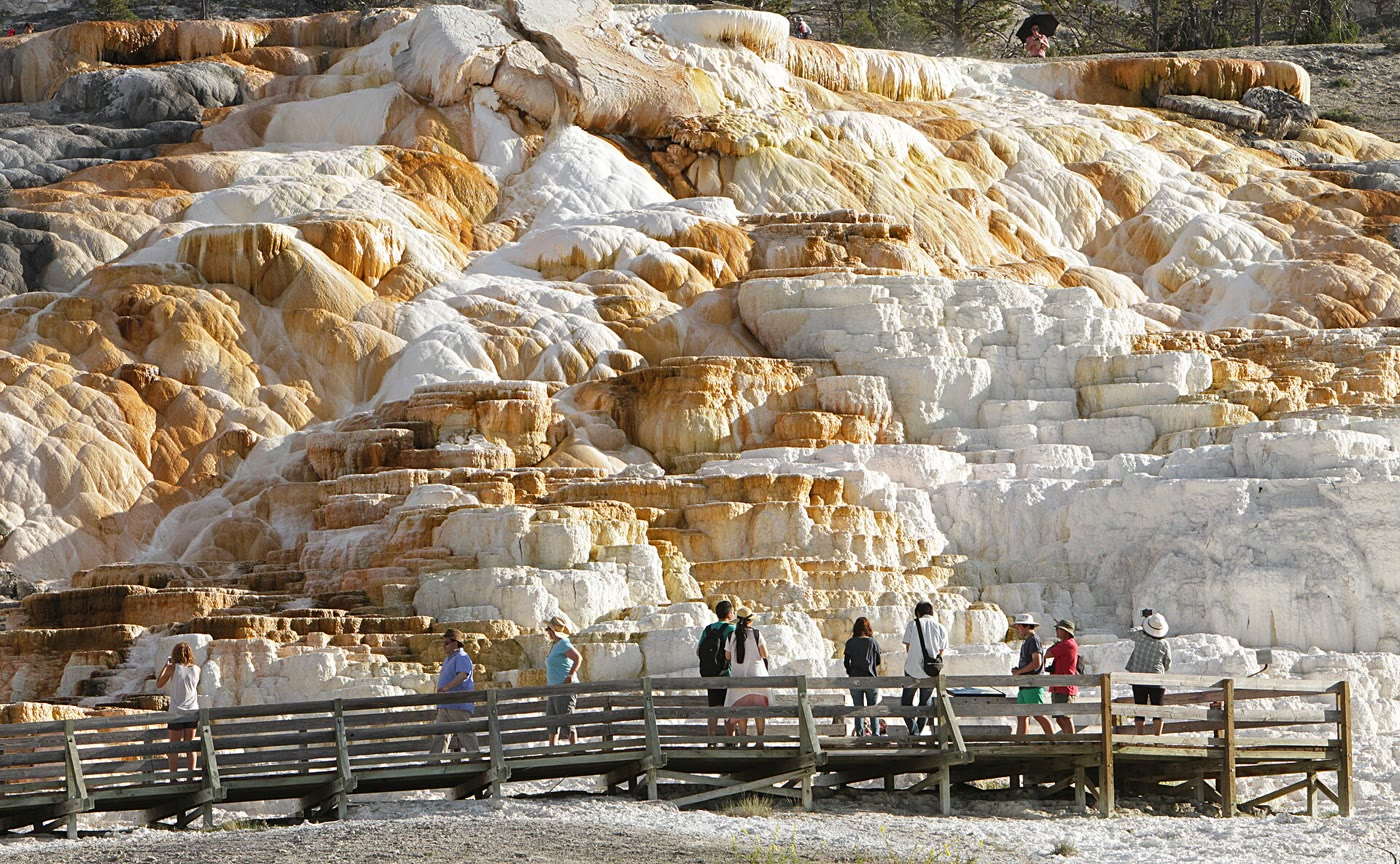
\includegraphics[width=\linewidth]{images/book5/b3-palette-spring-travertine.jpg}

{\scriptsize 猛犸热泉的调色板泉石灰华阶地，附
游步道与游客以示比例。NPS 照片，Jim Peaco 摄，公有领域。}
\end{minipage}
\end{inthefield}
% ledger: photo:b3-palette-spring, usgsyvo:travertine, nps:travertine-terraces

\section{硅酸盐风化动力学}\label{sec:b3:water-rock-interaction:kinetics}

硅酸盐的溶解远比方解石缓慢，水体很少
与之达到平衡，因此其溶解必须用速率来描述。

\begin{definition}[矿物溶解速率定律]\label{def:b3:water-rock-interaction:rate-law}
\emph{矿物溶解速率定律}\index{矿物溶解速率定律}给出单位矿物表面的溶解速率，
单位为
\unit{mol.m^{-2}.s^{-1}}，以对酸性、中性和碱性机制求和的形式表示，
\[
r = \sum_j k_j\,e^{-\frac{E_j}{R}\left(\frac1T - \frac1{298.15}\right)}\,
a_{\ce{H+}}^{n_j}\,\bigl(1 - \Omega^{p_j}\bigr)^{q_j},
\]
式中 $k_j$ 为 \qty{25}{\celsius} 时的速率常数，$E_j$ 为活化能，
$n_j$ 为反应级数（碱性机制中取负值），以及两个指数
$p_j$、$q_j$，通常取为 1。
\end{definition}
% ledger: pk04:rate-law

\begin{proposition}[远离平衡与接近平衡]\label{prop:b3:water-rock-interaction:affinity}
若 $p = q = 1$，则在 $\Omega \ll 1$ 时，速率不依赖于水的饱和度，
接近平衡时则与\omterm{def:b3:water-rock-interaction:si}{饱和指数}成正比，
即 $r \approx -2.303\,r_\infty\,\mathrm{SI}$，其中
$r_\infty$ 为远离平衡时的速率。
\end{proposition}

\begin{proof}
因子为 $1 - \Omega = 1 - 10^{\mathrm{SI}}$。当 $\mathrm{SI} \ll 0$ 时它
趋于 1；当 $\mathrm{SI}$ 接近 0 时，$10^{\mathrm{SI}} \approx 1 +
2.303\,\mathrm{SI}$。
\end{proof}

速率常数来自对新鲜矿物粉末所作的实验室实验，
实验在远离平衡的流通式反应器中进行。下图给出
四种矿物在 \qty{25}{\celsius} 时的速率方程。每条曲线呈
V 形或 U 形：质子加速酸性水中的溶解，氢氧根加速碱性水中的溶解，二者之间
由中性机制设定一个下限。橄榄石的溶解速率约
在 pH 5 时比钠长石快三个数量级，这正是它成为
土壤中最先消失的常见硅酸盐之一。钠长石与镁橄榄石的
活化能为 65 至 \qty{79}{kJ/mol}，使它们在 \qty{25}{\celsius} 时的速率
比 \qty{10}{\celsius} 时快四至五倍。
% ledger: pk04:rates

野外速率低得多，相差数个数量级。在柱实验中，对一块
新鲜碾碎的花岗岩，斜长石的速率在六年间持续
下降，至 \qty{7.0e-14}{mol.m^{-2}.s^{-1}}；同一花岗岩经自然风化，
并部分转变为高岭石后，溶解速率为 \qty{2.1e-15}{mol.m^{-2}.s^{-1}}，
相同条件下，两者仍远快于
风化剖面本身测得的速率。综合许多矿物与不同年龄的结果，
速率随矿物已风化的时间 $t$ 增加而下降，即 $R =
\num{3.1e-13}\,t^{-0.61}$（mol\,m$^{-2}$\,s$^{-1}$，$t$ 以年计）。部分
下降来自矿物本身，其中最活跃的表面先溶解；
其余则来自环境：水流缓慢，矿物多而流体少，
孔隙水接近平衡，依上述命题，速率
很小。
% ledger: whitebrantley03:rates

\begin{omfigure}
\begin{tikzpicture}
\begin{axis}[omrecord, width=0.74\linewidth, height=0.46\linewidth,
  xlabel={pH}, ylabel={$\log r$ (\unit{mol.m^{-2}.s^{-1}})},
  xmin=0, xmax=14, ymin=-14.5, ymax=-6, clip=false,
  xtick={0,2,4,6,8,10,12,14}, ytick={-14,-12,-10,-8,-6},
  yticklabels={$-14$,$-12$,$-10$,$-8$,$-6$},
  tick label style={font=\scriptsize}, label style={font=\small},
  legend style={font=\scriptsize, legend cell align=left, at={(1.03,0.5)}, anchor=west}]
% computed in figdata/bachelor-3/weathering_rates.py
\addplot[green!45!black, thick] table[x=ph, y=forsterite] {figdata/out/bachelor-3-weathering_rates-curves.dat};
\addlegendentry{镁橄榄石}
\addplot[omDef, thick] table[x=ph, y=albite] {figdata/out/bachelor-3-weathering_rates-curves.dat};
\addlegendentry{钠长石}
\addplot[red!70!black, thick, densely dashed] table[x=ph, y=kfeldspar] {figdata/out/bachelor-3-weathering_rates-curves.dat};
\addlegendentry{钾长石}
\addplot[black, thick, densely dotted] table[x=ph, y=kaolinite] {figdata/out/bachelor-3-weathering_rates-curves.dat};
\addlegendentry{高岭石}
\end{axis}
\end{tikzpicture}

\par\smallskip{\small 远离平衡时的溶解速率，在
\qty{25}{\celsius} 下随 pH 的变化，取自已发表的实验室
速率参数汇编。橄榄石端元镁橄榄石在该汇编中无碱性机制，
其曲线在中性下限处即停止下降。}\label{fig:b3:water-rock-interaction:rates}
\end{omfigure}
% ledger: pk04:rates

\begin{definition}[风化机制]\label{def:b3:water-rock-interaction:regimes}
地表的化学风化处于\emph{供给限制型}\index{供给限制型}状态，指其速率受
侵蚀把新鲜矿物带到风化锋的速率所限制；
新鲜矿物充足时，则为
\emph{风化限制型}\index{风化限制型}状态，
其速率受反应本身限制。
\end{definition}

对一批小流域的汇编表明两种状态都存在。侵蚀缓慢处，
土层厚且经淋滤，地形平缓，风化通量跟随
侵蚀速率变化：任何到达的新鲜岩石都被充分淋滤，气候变暖或
变湿几乎不起作用。侵蚀迅速处，如陡峭的山地，通量
随径流增大，大致与侵蚀速率的平方根成正比，并随温度升高而增大，
表观活化能为 $74 \pm
\qty{29}{kJ/mol}$。只有在第二种状态下，硅酸盐风化才能充当
本科二年级分册中所述的气候恒温器。
% ledger: west05:regimes

水在风化时形成哪种次生矿物，要在另一
张图上读取。

\begin{definition}[活度图]\label{def:b3:water-rock-interaction:activity-diagram}
\emph{活度图（矿物稳定性）}\index{活度图（矿物稳定性）}
把水的活度比平面（例如
$\log(a_{\ce{K+}}/a_{\ce{H+}})$ 对 $\log a_{\ce{H4SiO4}}$）划分为
化学体系中每种矿物各自为稳定相的区域。
\end{definition}

\begin{proposition}[活度图的边界]\label{prop:b3:water-rock-interaction:boundaries}
在体系 \ce{K2O}--\ce{Al2O3}--\ce{SiO2}--\ce{H2O} 中，固相中的铝守恒，
水的活度取为 1。设某矿物每化学式含 $k$ 个钾原子、$a$ 个铝原子、
$s$ 个硅原子，溶解常数为 $K$（溶解产物为 \ce{K+}、
\ce{Al^3+}、\ce{H4SiO4}），则
\[
\log\frac{a_{\ce{Al^3+}}}{a_{\ce{H+}}^3} = \frac{\log K - kX - sY}{a},
\qquad X = \log\frac{a_{\ce{K+}}}{a_{\ce{H+}}},\quad Y = \log a_{\ce{H4SiO4}}.
\]
稳定矿物给出最低的铝活度，两种矿物之间的边界
在 $(Y, X)$ 平面中为一条直线。
\end{proposition}

\begin{proof}
溶解过程由电荷平衡消耗 $h = k + 3a$ 个质子，故 $a\log
a_{\ce{Al^3+}} = \log K + h\log a_{\ce{H+}} - k\log a_{\ce{K+}} - s\log
a_{\ce{H4SiO4}}$；两边除以 $a$，并将 $3\log a_{\ce{H+}}$ 移到左边，
即得所求表达式。与某一矿物达到平衡的水
对于需要更多铝的任何矿物是未饱和的，对于需要更少铝的
任何矿物则是过饱和的，因此溶解度最小者为
稳定相。令两个这样的表达式相等，它们关于 $X$ 和 $Y$ 都是线性的，于是得到一条直线。
\end{proof}

取 \qty{25}{\celsius} 下的常数，三水铝石让位于高岭石的条件为
$\log a_{\ce{H4SiO4}} = -4.39$（即 \qty{2.4}{mg/L} 的二氧化硅），高岭石让位于白云母的条件为
$\log(a_{\ce{K+}}/a_{\ce{H+}}) = 1.55$，钾长石只
在富含钾和硅的水中稳定。该图是本科一年级分册中风化序列的
数值版本：稀薄的水把钾和硅冲走，
使长石分解到只剩三水铝石；保留更多硅的水
形成高岭石；保留更多钾的水（如在深部），
则形成云母。
% ledger: phreeqc:silicates

\begin{omfigure}
\begin{tikzpicture}
\begin{axis}[omrecord, width=0.66\linewidth, height=0.5\linewidth,
  xlabel={$\log a_{\ce{H4SiO4}}$}, ylabel={$\log(a_{\ce{K+}}/a_{\ce{H+}})$},
  xmin=-6, xmax=-2, ymin=0, ymax=10, clip=false,
  xtick={-6,-5,-4,-3,-2}, xticklabels={$-6$,$-5$,$-4$,$-3$,$-2$},
  tick label style={font=\scriptsize}, label style={font=\small}]
% computed in figdata/bachelor-3/activity_diagram.py
\addplot[black, thick, unbounded coords=jump] table[x=y, y=x] {figdata/out/bachelor-3-activity_diagram-lines.dat};
\addplot[omDef, densely dashed] table[x=y, y=x] {figdata/out/bachelor-3-activity_diagram-quartz.dat};
\addplot[omDef, densely dotted] table[x=y, y=x] {figdata/out/bachelor-3-activity_diagram-amorph.dat};
\addplot[red!70!black, only marks, mark=*, mark size=1.8pt] table[x=y, y=x] {figdata/out/bachelor-3-activity_diagram-samples.dat};
\node[font=\small] at (axis cs:-5.4,0.8) {三水铝石};
\node[font=\small] at (axis cs:-3.25,0.75) {高岭石};
\node[font=\small] at (axis cs:-4.6,5.0) {白云母};
\node[font=\small] at (axis cs:-3.3,9.3) {钾长石};
\node[font=\scriptsize, omDef, anchor=south] at (axis cs:-3.98,10) {石英};
\node[font=\scriptsize, omDef, anchor=south] at (axis cs:-2.71,10) {无定形二氧化硅};
\node[font=\scriptsize, red!70!black, anchor=west] at (axis cs:-4.58,0.38) {A};
\node[font=\scriptsize, red!70!black, anchor=west] at (axis cs:-3.80,1.29) {B};
\node[font=\scriptsize, red!70!black, anchor=west] at (axis cs:-3.48,4.08) {C};
\end{axis}
\end{tikzpicture}

\par\smallskip{\small 体系中的稳定区域，
\ce{K2O}--\ce{Al2O3}--\ce{SiO2}--\ce{H2O} 在 \qty{25}{\celsius} 下，图中标出石英
（虚线）与无定形二氧化硅（点线）的饱和线。三种虚构的水：A，稀薄的
热带溪流；B，流经花岗岩的溪流；C，
花岗岩中的深层地下水。}\label{fig:b3:water-rock-interaction:activity}
\end{omfigure}
% ledger: phreeqc:silicates

\section{热液流体}\label{sec:b3:water-rock-interaction:hydrothermal}

热水沿地壳循环，靠近洋中脊或侵入体时，
会与所经过的岩石交换氧。高温下，
岩石与水之间的分馏很小，两者都趋向
同位素平衡：大气降水较轻，使岩石变轻，
使水变重。岩石移动的距离，量度了有多少水
已经通过。

\begin{definition}[水岩比]\label{def:b3:water-rock-interaction:water-rock-ratio}
热液体系的\emph{水岩比}\index{水岩比} $W/R$ 是
与一定质量岩石发生交换的水的质量，
除以该岩石的质量。
\end{definition}

\begin{proposition}[由氧同位素求水岩比]\label{prop:b3:water-rock-interaction:wr}
设初始 $\delta_r^i$ 的岩石与初始
$\delta_w^i$ 的水交换氧，直至达到 $\delta_r^f$，并与其最后接触的水处于平衡，
$\Delta = \delta_r^f - \delta_w^f$，又设 $c_r$ 与 $c_w$ 分别为
岩石和水中的氧浓度。在封闭体系（一批水）
与开放体系（水经过一次）中，
\[
\frac WR\Big|_{\text{封闭}} = \frac{c_r}{c_w}\,
\frac{\delta_r^f - \delta_r^i}{\delta_w^i - \delta_r^f + \Delta},
\qquad
\frac WR\Big|_{\text{开放}} = \frac{c_r}{c_w}\,
\ln\!\left(\frac{\delta_r^f - \delta_r^i}{\delta_w^i - \delta_r^f + \Delta} + 1\right).
\]
\end{proposition}

\begin{proof}
封闭体系：氧-18 守恒，$c_wW\delta_w^i + c_rR\delta_r^i = c_wW
\delta_w^f + c_rR\delta_r^f$，其中 $\delta_w^f = \delta_r^f - \Delta$，解
出 $W/R$。开放体系中，一份水 $\mathrm dW$ 以 $\delta_w^i$ 进入，
与岩石平衡后以 $\delta_r - \Delta$ 离开，故 $c_rR\,\mathrm d\delta_r
= c_w(\delta_w^i - \delta_r + \Delta)\,\mathrm dW$。分离变量得
$\int_{\delta_r^i}^{\delta_r^f}\mathrm d\delta_r/(\delta_w^i - \delta_r +
\Delta) = (c_w/c_r)\,W/R$，而积分为 $-\ln[(\delta_w^i - \delta_r^f
+ \Delta)/(\delta_w^i - \delta_r^i + \Delta)]$，即所求表达式。
\end{proof}

对于氧，$c_r/c_w$ 接近 0.5。在相同位移下，开放体系所需的水量总是
少于封闭体系，因为每一份水离开时都尽可能“重”。
在许多侵入体周围，围岩的 $\delta^{18}\mathrm O$ 呈现低值的靶心状分布，
从约 $+6$ 降至 0 以下，
中心位于流经水量最多之处；热液流体的矿石常常
位于最低等值线之内，这使得该图成为
一种找矿工具。
% ledger: white13c9:water-rock

\begin{omfigure}
\begin{tikzpicture}[font=\small, >=Stealth]
\draw[thick, fill=black!6] (0,0) rectangle (4,2.2);
\node at (2,1.55) {岩石，质量 $R$};
\node at (2,0.95) {$\delta_r^i \to \delta_r^f$};
\node[font=\scriptsize] at (2,0.4) {温度 $T$ 下交换};
\draw[->, thick, omDef] (-2.6,1.1) -- (-0.1,1.1);
\node[omDef, anchor=south, align=center, font=\scriptsize] at (-1.35,1.15) {进入的水 \\ $\delta_w^i$，$\mathrm dW$};
\draw[->, thick, red!70!black] (4.1,1.1) -- (6.6,1.1);
\node[red!70!black, anchor=south, align=center, font=\scriptsize] at (5.35,1.15) {流出的水 \\ $\delta_r - \Delta$};
\node[anchor=north, font=\scriptsize, align=center] at (2,-0.15) {开放体系：每份水只流经一次，\\ 以与其最后接触的岩石平衡之态流出};
\end{tikzpicture}

\par\smallskip{\small 热液体系的箱式模型。在封闭体系中，
一批水与岩石共处，直至二者达到平衡；
在开放体系中水持续流过，岩石随每一份水
略微向水的组成方向转移。}\label{fig:b3:water-rock-interaction:box}
\end{omfigure}

\begin{definition}[反应路径模型]\label{def:b3:water-rock-interaction:reaction-path}
\emph{反应路径模型}\index{反应路径模型}追踪水的组成及其形成的矿物
随反应进行的变化，
其做法是逐步加入少量反应物（矿物溶解、气体逸出、
移除热量），并在每一步重新计算形态及\omterm{def:b3:water-rock-interaction:si}{饱和指数}，
使任何达到饱和的矿物沉淀。
\end{definition}

将\omterm{def:b3:water-rock-interaction:reaction-path}{反应路径模型}用于周末问题中的泉水并逐步脱气时，
一旦方解石的\omterm{def:b3:water-rock-interaction:si}{饱和指数}超过零即沉淀出方解石；若用于
一种花岗岩与一种雨水，则先形成三水铝石，再形成高岭石，然后
形成云母；水中二氧化硅与钾不断积累，在
活度图上描出一条路径。形态计算程序借助平衡常数数据库完成这些计算，
其数据库中的平衡常数例如本章所用的那些。
% ledger: phreeqc:silicates

\section{练习}

\begin{exercise}[$\star$]\label{exo:b3:water-rock-interaction:1}
某水体中（单位为 \unit{mg/L}）含 \ce{Ca} 48、\ce{Mg} 9.7、\ce{Na} 23、\ce{K} 3.9、
\ce{HCO3} 183、\ce{Cl} 35.5 和 \ce{SO4} 48。求其电荷平衡
误差，判断该分析是否可接受。
\end{exercise}

\begin{exercise}[$\star$]\label{exo:b3:water-rock-interaction:2}
离子强度为 0.0050 时，求
\ce{Ca^2+}、\ce{HCO3-} 和 \ce{SO4^2-} 的活度系数。
\end{exercise}

\begin{exercise}[$\star$]\label{exo:b3:water-rock-interaction:3}
某水流经含石膏的泥灰岩，水中含钙 \qty{3.0}{mmol/L}，
硫酸根 \qty{4.0}{mmol/L}，离子强度为 0.016。求
石膏的\omterm{def:b3:water-rock-interaction:si}{饱和指数}，并判断该水能否继续溶解石膏？
\end{exercise}

\begin{exercise}[$\star$]\label{exo:b3:water-rock-interaction:4}
某地下水含二氧化硅 \qty{12}{mg/L}（以 \ce{SiO2} 计），
以 \ce{H4SiO4} 形式存在，求其对石英的\omterm{def:b3:water-rock-interaction:si}{饱和指数}及
无定形二氧化硅的\omterm{def:b3:water-rock-interaction:si}{饱和指数}，温度为 \qty{25}{\celsius}。
\end{exercise}
% ledger: phreeqc:silicates

\begin{exercise}[$\star\star$]\label{exo:b3:water-rock-interaction:5}
取活度系数为 1，求一开放体系溶解的钙量，
其中 $P_{\ce{CO2}} = 10^{-2}$~atm，温度分别为 \qty{25}{\celsius} 与
\qty{10}{\celsius}，分别以 \unit{mmol/L} 和 \unit{mg/L} 计。
\end{exercise}

\begin{exercise}[$\star\star$]\label{exo:b3:water-rock-interaction:6}
某水体温度为 \qty{25}{\celsius}，pH 为 7.60，
并含碳酸氢根 \qty{4.0}{mmol/L}。取活度系数为 1，求其溶解的二氧化碳
和碳酸根、$P_{\ce{CO2}}$，以及各形态在
溶解无机碳中所占的份额。
\end{exercise}

\begin{exercise}[$\star\star$]\label{exo:b3:water-rock-interaction:7}
一颗钠长石颗粒为直径 \qty{1}{mm} 的球体，位于 pH 为 5 的土壤水中，温度为
\qty{25}{\celsius}，按图中给出的速率溶解，$\log r = -12.09$。
已知摩尔体积为 \qty{101.31}{cm^3/mol}，求其半径
缩小的速率，并求其可持续多长时间。
\end{exercise}
% ledger: pk04:rates, phreeqc:silicates

\begin{exercise}[$\star\star$]\label{exo:b3:water-rock-interaction:8}
求钠长石的中性溶解速率（$E =
\qty{69.8}{kJ/mol}$）从 \qty{5}{\celsius} 升至 \qty{25}{\celsius} 时
增大到原来的多少倍？并求 $E = \qty{74}{kJ/mol}$ 的风化通量的倍数。
\end{exercise}
% ledger: pk04:rates, west05:regimes

\begin{exercise}[$\star\star$]\label{exo:b3:water-rock-interaction:9}
由以下平衡常数推导活度图中高岭石–白云母的边界，
所用常数为 $\log K = 7.435$（高岭石，2 Al，2 Si）和 $12.703$（白云母，1
K，3 Al，3 Si）。某水体温度为 \qty{25}{\celsius}，含钾 \qty{2.0}{mg/L}，
二氧化硅 \qty{15}{mg/L}，pH 为 7.0：它会形成哪种矿物？
\end{exercise}
% ledger: phreeqc:silicates

\begin{exercise}[$\star\star\star$]\label{exo:b3:water-rock-interaction:10}
靠近侵入体处发现一块花岗闪长岩，其 $\delta^{18}\mathrm O = +6$，
实测为 $-2$（\unit{\permil}）。大气降水为 $-13$，在
交换温度下，岩石比水重 \qty{2}{\permil}，
在 $c_r/c_w = 0.5$ 时，分别计算封闭系统和
开口系统的\omterm{def:b3:water-rock-interaction:water-rock-ratio}{水岩比}，并解释二者为何不同。
\end{exercise}
% ledger: white13c9:water-rock

\begin{exercise}[$\star\star\star$]\label{exo:b3:water-rock-interaction:11}
降雨携带土壤气，其 $P_{\ce{CO2}} = 10^{-1.5}$~atm，
温度为 \qty{10}{\celsius}，到达一石灰岩层。取活度系数均为 1，
分别计算两种情形下溶解的钙：一是保持与土壤气连通，
二是先将其与之隔离。其二氧化碳剩余的比例为多少，
在封闭情形下，并求其最终的 $P_{\ce{CO2}}$？
\end{exercise}

\begin{exercise}[$\star\star\star$]\label{exo:b3:water-rock-interaction:12}
利用近平衡速率的命题，求矿物溶解速率占其
远离平衡速率的比例，当 $\mathrm{SI} =
-2$、$-1$ 和 $-0.1$ 时各为多少？
实验室测得反应 6 年后的速率遵循本章的幂律，
问经过 \num{10000} 年后其速率将下降多少倍？综合两种效应，
解释野外速率为何如此低。
\end{exercise}
% ledger: whitebrantley03:rates

\section{问题：瓦尔登石灰岩之下的泉}

\begin{problem}[{周末问题——一处虚构石灰岩泉的分析、二氧化碳与饱和度，
以及一条花岗岩溪流}]
\label{pb:b3:water-rock-interaction:1}
一处泉水涌出于瓦尔登丘陵的侏罗纪石灰岩山脚，
温度为 \qty{10}{\celsius}，pH 为 7.20。其分析结果（单位 \unit{mg/L}）如下：\ce{Ca}
112、\ce{Mg} 4.0、\ce{Na} 7.0、\ce{K} 1.2、\ce{HCO3} 340、\ce{Cl} 11、
\ce{SO4} 14、\ce{NO3} 9。在 \qty{10}{\celsius} 下：$\log K_{\mathrm{cal}} =
-8.35$，$\log K_1 = -6.46$，$\log K_2 = -10.49$，$\log K_H = -1.27$。取本章的
扩展德拜–休克尔方程，忽略离子对，并取
大气的 $\log P_{\ce{CO2}} = -3.37$。

\medskip\noindent\textbf{第一部分——分析。}
\begin{enumerate}
\item 将分析结果换算为 \unit{mmol/L}。
\item 计算电荷平衡误差，分析结果是否可接受？
\item 计算离子强度。
\item 计算 \ce{Ca^2+}、\ce{HCO3-} 和
  \ce{CO3^2-} 的活度系数。
\item 此处扩展德拜–休克尔方程是否适用？
\end{enumerate}

\medskip\noindent\textbf{第二部分——二氧化碳。}
\begin{enumerate}[resume]
\item 计算碳酸氢根的活度。
\item 计算溶解二氧化碳的活度。
\item 计算泉水的 $P_{\ce{CO2}}$，它是大气的多少倍，
  二氧化碳可能来自何处？
\item 计算碳酸根浓度，以及各物种
  在溶解无机碳中所占的比例。
\item 检验碱度几乎全部来自碳酸氢根。
\end{enumerate}

\medskip\noindent\textbf{第三部分——饱和度与钙华。}
\begin{enumerate}[resume]
\item 计算方解石的离子活度积和\omterm{def:b3:water-rock-interaction:si}{饱和指数}，
  取出口处的数值。
\item 泉水是否与方解石达到平衡？它是管道泉还是
  缓慢分散渗出的泉？
\item 计算与方解石平衡的开口系统中的钙离子浓度，
  取泉水的 $P_{\ce{CO2}}$，活度系数取第 4 题的值，
  并与分析结果比较。
\item 水在任何方解石形成之前脱气进入大气。保持
  碳酸氢根活度不变，计算其 pH 值和\omterm{def:b3:water-rock-interaction:si}{饱和指数}。
\item 估算其沉淀方解石、恢复至与大气平衡后，
  保留的钙（开口系统，活度系数取新离子强度
  $3m$ 时的值），以及每升方解石的质量。
\item 泉水流量为 \qty{2.0}{L/s}，其沉积物分布于
  \qty{400}{m^2} 的面积上。若所有方解石都留在此处，密度为
  \qty{2.71}{g/cm^3}，沉积物将以多快的速度增长？
\end{enumerate}

\medskip\noindent\textbf{第四部分——花岗岩溪流。}一条溪流位于
瓦尔登花岗岩之上，地表覆盖厚层土壤、坡度平缓，其（
\qty{25}{\celsius}）下，钾为 \qty{1.2}{mg/L}，\qty{9.0}{mg/L} 的
二氧化硅，pH 为 5.8。
\begin{enumerate}[resume]
\item 计算其在活度图上的位置。
\item 它会形成哪种矿物？计算其对石英的\omterm{def:b3:water-rock-interaction:si}{饱和指数}。
\item 二氧化硅浓度低于多少时会形成三水铝石？
\item pH 为多少时，它会到达高岭石–白云母边界？
\item 计算钾长石在该水中远离
  平衡时的溶解速率，由参数 $\log k = -10.06$、$n = 0.500$（酸性）；
  $-12.41$（中性）；$-21.20$，$n = -0.823$（碱性）。
\item 该流域的风化更可能属于\omterm{def:b3:water-rock-interaction:regimes}{供给限制型}还是
  \omterm{def:b3:water-rock-interaction:regimes}{风化限制型}？为什么？
\item 取表观活化能为 \qty{74}{kJ/mol}，\omterm{def:b3:water-rock-interaction:regimes}{风化限制型}通量
  在 \qty{10}{\celsius} 与
  \qty{25}{\celsius} 之间变化了多少倍？
\item 写出泉水在其
  出口处的方解石\omterm{def:b3:water-rock-interaction:si}{饱和指数}。
\end{enumerate}
\end{problem}
% ledger: phreeqc:carbonate, phreeqc:silicates, hem85:debye-huckel, hem85:charge-balance, hem85:si, hem85:pco2, pk04:rates, west05:regimes, data:co2-mlo
